\subsection{Small batches change the competitive region}
\label{sec:7-smallbatch}

T5 compares scheduled JHQ, CAGRA fp32/int8 and IVF-RaBitQ at batches
8/32 on the four E1 datasets. Five synchronous host-to-host rounds use
1,000/992 queries, respectively. Its 1,808 points include JHQ's one-block
control; IVF-PQ and brute force are outside this campaign.
\Cref{fig:7-smallbatch,tab:7-smallbatch} compare the resulting regions.

\suppressfloats[t]
\begin{figure}[htbp]
\centering
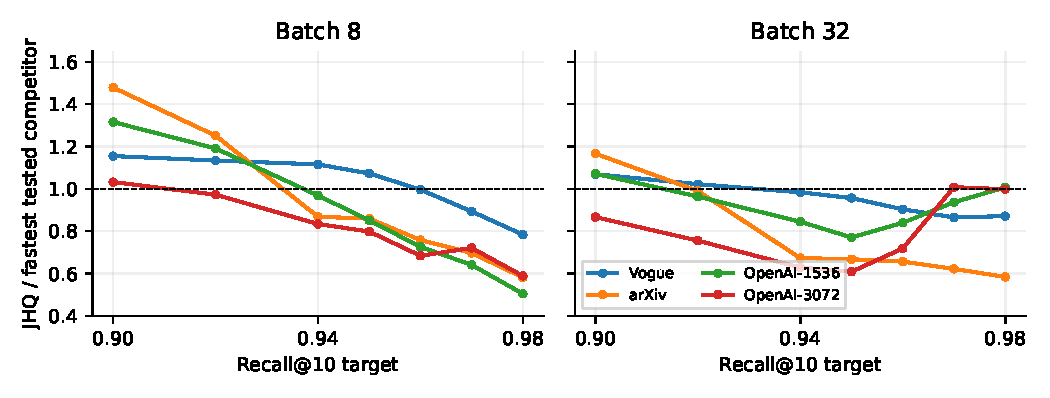
\includegraphics[width=\linewidth]{t4-t5/smallbatch.pdf}
\caption[Small-batch competitive regions]{T5 JHQ / fastest-competitor
QPS under interpolation with qualifying measured endpoints. Above one
favours JHQ. Strict measured thresholds are in \cref{tab:7-smallbatch}.}
\label{fig:7-smallbatch}
\end{figure}

\begin{table}[htbp]
\centering
\caption[Small-batch matched-recall ratios]{T5 QPS ratios:
interpolation with qualifying endpoints / strict measured threshold.
The fastest competitor is selected independently for each estimator;
higher-recall qualifying endpoints remain eligible without extrapolation.}
\label{tab:7-smallbatch}
\footnotesize\setlength{\tabcolsep}{4pt}
\begin{tabular}{@{}lrrrr@{}}
\toprule
Dataset & $b$ & $R=0.90$ & $R=0.95$ & $R=0.97$ \\
\midrule
Vogue & 8 & 1.155 / 1.091 & 1.073 / 0.980 & 0.893 / 0.854 \\
Vogue & 32 & 1.069 / 0.997 & 0.956 / 0.895 & 0.865 / 0.839 \\
arXiv & 8 & 1.479 / 1.454 & 0.859 / 0.851 & 0.697 / 0.698 \\
arXiv & 32 & 1.166 / 1.148 & 0.667 / 0.661 & 0.622 / 0.582 \\
OpenAI-1536 & 8 & 1.316 / 1.131 & 0.851 / 0.825 & 0.641 / 0.620 \\
OpenAI-1536 & 32 & 1.071 / 0.915 & 0.770 / 0.752 & 0.937 / 0.914 \\
OpenAI-3072 & 8 & 1.032 / 0.953 & 0.798 / 0.798 & 0.721 / 0.702 \\
OpenAI-3072 & 32 & 0.866 / 0.734 & 0.608 / 0.771 & 1.008 / 1.351 \\
\bottomrule
\end{tabular}

\end{table}

At recall 0.97 and batch 8, CAGRA fp32 leads on all four datasets under
both estimators: interpolated JHQ ratios are 0.641--0.893. At batch 32,
these ratios are 0.622--1.008, with OpenAI-3072 close under interpolation
but favourable to JHQ under the measured threshold. At recall 0.95,
Vogue's batch-8 lead likewise appears only under interpolation. Grid
resolution therefore matters to borderline rankings.

Lower-recall comparisons must retain competitors whose fastest frontier
point already exceeds the target.
At 0.90, corrected interpolated ratios are 1.032--1.479 at batch 8 and
0.866--1.166 at batch 32; the strict measured estimator gives three
and one JHQ wins, respectively. Omitting qualifying endpoints would
overstate these low-recall leads.
Scheduling is still useful: at recall 0.95 its interpolated gain over
one block is 1.7--3.3$\times$. An internal execution gain therefore need
not produce a cross-system lead.

Null-call medians by dataset, method and batch span 0.012--0.072\,ms;
this overhead remains in search timing. CAGRA uses Python bindings, while JHQ/RaBitQ use C++;
warm-up policies also differ. Protocol and grid details are in \cref{sec:a-t4-t5}. E1's full-batch
high-recall leads do not generalise to these small batches.
